\documentclass{article}

\usepackage[hscale=0.8,vscale=0.8]{geometry}
\usepackage{graphicx}
\usepackage{amsfonts, amsmath, amsthm, amssymb} % For math fonts, symbols and environments



\pagenumbering{gobble}

\author{Finnian Lattimore}
\title{Causal Inference in one page}

\begin{document}
\def\ci{\perp\!\!\!\perp}
\setlength\parindent{0pt}
\subsection*{Causal Inference}
Causal inference covers problems where we want to predict the outcome of an intervention given some known causal structure
\begin{itemize}
\item Assume that the true causal structure is a directed graphical model where $X \rightarrow Y$ means $X$ causes $Y$. We know the structure of the network but may not be able to observe the values of all the variables.
\item Intervening to set $X = x$, denoted $do(X=x)$ in a causal network, has the effect of removing all links coming into the variable $X$ (since its value is no longer determined by its parents) and setting its value to $x$.
\item We can use d-separation to derive the 3 rules of the do-calculus that allow us write queries about interventions in terms of the pre-interventional distribution. 
\item These rules are complete.  If an expression containing do's can be converted into one that does not by repeated application of the rules then you can determine the post-interventional distribution from observational data. If you can't, its not possible without additional assumptions.
\end{itemize}
The rules (simplified to cover only the case where we intervene on a single variable) can all be illustrated by the graph in figure \ref{fig:dorules}. Assume our query is $P(Y|do(X))$. $G^{\dagger}$ is the original graph, $G$, augmented to include a variable $\hat{X}$  that acts as a switch determining if $X$ takes its value as determined by its parents or from an external intervention. $G_{\overline{X}}$ is $G$ after the intervention. 

\begin{figure}[h]
\caption{The do calculus}
\label{fig:dorules}
\centering
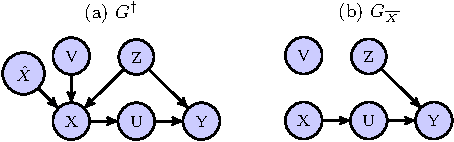
\includegraphics[scale=0.9]{do_rules_figure-crop}
\end{figure}

\begin{enumerate}
\item D-separation still applies after an intervention. $Y \ci V|X$ in $G_{\overline{X}}$ $\implies P(Y|do(X),V) = P(Y|do(X))$
\item If the outcome variable is independent of the way in which the intervened on variable takes its value, intervention = observation. $Y \ci \hat{X}|X,Z$ in $G^{\dagger} \implies P(Y|do(X),Z) = P(Y|X,Z)$
\item If there is no direct path from the intervened on variable to the outcome variable, the intervention does not effect the distribution of the outcome variable. $Y \ci \hat{X}|U,Z$ in  $G^{\dagger} \implies P(Y|do(X),U,Z) = P(Y|U,Z)$ (note: we condition on $Z$ because conditioning on $U$ opens the path $\hat{X} \leftarrow Z \rightarrow Y$)
\end{enumerate}

A single application of the rules show we can identify the causal effect of $X$ on $Y$ if we can observe $Z$. By repeated application of the rules the query is also identifiable if we can observe only $U$.


Key general references: \cite{Pearl2000,Koller2009}

\subsection*{Causal Structure Learning - learn causal structure from observational data}
\subsubsection*{Conditional independence approach} 

\begin{itemize}
\item Assume that the data was generated by an unknown causal directed graphical model
\item Assume that all dependencies in the graph are reflected by conditional dependencies in the distribution of the data (ie no dependencies exactly cancel one-another out) $\leftarrow$ faithfullness assumption
\item Finding the true causal structure is equivalent to finding the set of graphs that are perfect maps for the data distribution. In general, result is not unique but some links may have the same direction in all graphs in the set.
\item Approach can be extended to allow for latent variables
\item Key general reference: \cite{Sprites}
\end{itemize}
\subsubsection*{Functional form approach}
Conditional independence based methods cannot distinguish between graphs with the same dependency structure, for example,  $X \rightarrow Y$ vs $Y \rightarrow X$. We can infer causality in such cases if we make braod assumptions about the relationship between the function mapping cause to effect and any noise. Suppose $X \rightarrow Y$:
\begin{itemize}
\item If we assume noise is additive in the causal direction, $Y = f(X)+\epsilon$ cannot generally be inverted to give an additive model in the other direction (linear $f$ and gaussian $\epsilon$ are an unfortunate exception)\cite{Hoyer2009}.
\item If $f$ is deterministic and invertible, for most input distributions $p_X(x)$ the distribution of $p_Y(y)$ will be higher where $f'$ is small and a large region of $X$ maps to similar values of $Y$. We expect that $f$ and $p_X$ are independent but $f'$ and $p_Y$ are correlated \cite{Daniusis2010}.
\item In general, $P(X)$ and $P(Y|X)$ should be independent but $P(Y)$ and $P(X|Y)$ will not be \cite{Scholkopf2012}
\end{itemize}

\bibliographystyle{plain} % Plain referencing style
\bibliography{library} % Use the example bibliography file sample.bib
\end{document}